\documentclass[a4paper, 11]{report}
\usepackage{amssymb,amsmath}
\usepackage{url}
\usepackage[final]{listings}
\usepackage{verbatim}
\usepackage{fixme}
\usepackage{titlesec}
\usepackage{fancyhdr}
\usepackage{layout}
\usepackage{multirow}
\usepackage{multicol}
\usepackage{pgfplots}
\usepackage{array}
\usepackage{mdwmath}
\usepackage{mdwtab}
\usepackage{xcolor}
\usepackage{tikz}
\usepackage{geometry}
\usepackage{rotating}
\usepackage{pbox}
\usepackage{pdflscape}
\usepackage{tabularx}
%\usepackage{pstricks}
\usepackage{parskip}
\usepackage{algpseudocode}
\usepackage{algorithm}

\parskip 8pt

\usepackage{hyperref}
\hypersetup{
    colorlinks=false,
    pdfborder={0 0 0},
}


\usepackage{cleveref}
\listfiles

\graphicspath{{figs/}}
\setlength{\headheight}{15pt}

\definecolor{UniBlue}{RGB}{83,121,190}

\pagestyle{fancy}
\renewcommand{\chaptermark}[1]{ \markboth{#1}{} }
%\renewcommand{\sectionmark}[1]{ \markright{#1}{} }

%\fancyhf{}
\fancyhead[LE,RO]{\color{UniBlue}\thepage}
\fancyhead[RE]{\color{UniBlue}\nouppercase{\leftmark} }
\fancyhead[LO]{\color{UniBlue}\nouppercase{\rightmark} }

\fancypagestyle{plain}{ %
%  \fancyhf{} % remove everything
%  \renewcommand{\headrulewidth}{0pt} % remove lines as well
%  \renewcommand{\footrulewidth}{0pt}
}

% --- Commands ---
\newcommand{\HRule}{\rule{\linewidth}{0.2mm}}
\newcommand{\mailto}[1]{\href{mailto:#1}{\texttt{#1}}}
\newcommand{\XXX}[1]{{\bf \color{red} XXX: #1}}
\newcommand{\TODO}[0]{{\bf \color{red} TODO\ }}
\newcommand{\FAST}[0]{FAST}
\newcommand{\fastc}[0]{\texttt{fastc}}
\newcommand\reduline{\bgroup\markoverwith
  {\textcolor{red}{\rule[-0.5ex]{2pt}{0.4pt}}}\ULon}
\newcommand{\FIC}[1]{\reduline{#1}}
\newcommand{\blt}{\raise .2ex\hbox{\tiny$\bullet$ }}
\newcommand\acknowledgements[1]{
  \typeout{Acknowledgements}
  \thispagestyle{plain}
  \begin{center}{\huge{Acknowledgements} \par}\end{center}
      {\normalsize #1}
      \vfil\vfil\null
}
\newcommand\myabstract[1]{
  \typeout{Abstract}
  \thispagestyle{plain}
  \vspace{-3cm}
  \begin{center}{\huge{Abstract} \par}\end{center}
      {\normalsize #1}
      \vfil\vfil\null
}

\titleformat{\chapter}{\normalfont\Huge\bfseries\color{UniBlue}}{\thechapter}{1em}{}
\titleformat{\section}{\normalfont\Large\bfseries\color{UniBlue}}{\thesection}{1em}{}
\titleformat{\subsection}{\normalfont\large\bfseries\color{UniBlue}}{\thesubsection}{1em}{}


%\titlespacing*{\chapter}{0pt}{0pt}{10pt}

\newcounter{nodemarkers}
\newcommand\marktext[1]{%
  \tikz[overlay,remember picture]
  \node (marker-\arabic{nodemarkers}-a) at (0,1.5ex) {};%
  #1%
  \tikz[overlay,remember picture]
  \node (marker-\arabic{nodemarkers}-b) at (0,0){};%
  \tikz[overlay,remember picture,inner sep=2pt]
  \node[draw,dotted,rectangle,fit=(marker-\arabic{nodemarkers}-a.center) (marker-\arabic{nodemarkers}-b.center)] {};%
  \stepcounter{nodemarkers}%
}

% --- S ---

\usetikzlibrary{shapes,arrows,fit}
\usetikzlibrary{positioning}

% ---- Listings ----
\lstdefinestyle{lara}{ language=C++,
  morekeywords={aspectdef, var, apply, select, condition, begin, end, input}}

\lstdefinestyle{MaxC}{language=C++,
  morekeywords={s_int32, int32, float8_24, sin_float8_24,
    sout_float8_24, float8_24, s_int, s_float8_24, s_bool, in, out, count, countChain},
  deletekeywords={static}}

\lstdefinestyle{MaxJ}{
  morekeywords={HWVar, io, hwFloat, stream}
}


\lstset{aboveskip=20pt,
  belowskip=20pt,
  basicstyle=\small\sffamily,
  rulecolor=\color{lightgray},
  frame=single,
  frameround=tttt,
  keywordstyle=\color{black}\bfseries,
  numbers=left,
  numberstyle={\color{UniBlue}\scriptsize},
  captionpos=b,
  breaklines=true,
  xleftmargin=2em,
  escapeinside={(*@}{@*)}
}

\pgfplotsset{
  width=0.9\textwidth,
  enlargelimits=0.1,
  compat=1.8,
  tick label style={font=\footnotesize},
  label style={font=\footnotesize},
  legend style={font=\scriptsize},
  axis line style={lightgray},
}


\begin{document}

\begin{titlepage}

  \begin{center}

    {\Large Department of Computing, Imperial College London}
    \HRule \\[0.5cm]
    {\Large Custom Computing Research Group} \\[2cm]

    {\huge \bfseries Aspect Oriented Design for \\[0.25cm]Dataflow Engines}\\[0.5cm]
    {\Large -- Synopsis -- } \\[1.5cm]

    {\Large Paul Grigora\c{s}} \\[0.5cm]
    {\href{mailto:paul.grigoras09@imperial.ac.uk}{\texttt{\large paul.grigoras09@imperial.ac.uk}}}\\[1.5cm]

    \begin{figure}[!ht]
      \centering
      \def\svgwidth{0.6\linewidth}
      \input{figs/dataflow-cover.pdf_tex}
    \end{figure}
  \end{center}

\end{titlepage}


\renewcommand{\thepage}{\roman{page}}


\begin{abstract}
  \vspace{1em} Dataflow designs implemented on custom streaming
  architectures can be orders of magnitudes more efficient than
  traditional software, but they are developed with reduced
  productivity.  We propose a novel design flow for generating
  dataflow designs based on Aspect-oriented programming and explain
  how the proposed approach can be used to decouple design
  optimisation from design specification by encapsulating
  optimisations in separate aspect descriptions, which leads to
  improved productivity and efficiency. To support this approach we
  introduce a novel dataflow language that facilitates integration
  with existing aspect weaving tools and simplifies design development
  by supporting embedded hardware/software co-design, flexible number
  representation and run-time reconfiguration. We introduce novel
  aspect descriptions that specify system-level and implementation
  level optimisations strategies as well as strategies for improving
  developer productivity. We evaluate our approach on a number of
  applications, including advanced high-performance applications, such
  as the Reverse Time Migration technique for seismic imaging, and
  show that efficient dataflow designs up to 100 times faster than
  equivalent software only implementations can be derived with
  improved productivity.
\end{abstract}


\acknowledgements{

  I would like to thank:
\begin{itemize}
\item Professor Wayne Luk, for providing the inspiration for this
  project and guidance throughout
  \item Dr. Jose Gabriel Coutinho, for invaluable feedback and
    suggestions and including this work in the HARNESS project and
    providing the original source code for the Add Predictor kernel
  \item Xinyu Niu, for providing the original source code and
    background on the Reverse Time Migration and Black Scholes
    applications
  \item Dr. Timothy Todman and Dr. Stephen Weston, for providing
    constructive suggestions regarding the evaluation process
  \item Maxeler Technologies, especially Jacob Bower and Oliver Pell
    for their constructive suggestions on improving our paper and
    approach
  \item the anonymous reviewers of our paper for some interesting
    suggestions regarding future work
  \item my family and friends for their continuous support
\end{itemize}

}

\clearpage

\tableofcontents
\listoffigures
\listoftables
\lstlistoflistings

\pgfplotsset{width=0.7\textwidth, enlargelimits=0.15}

\renewcommand{\arraystretch}{1.5}

\section{Introduction}
We identify the following challenges:
\begin{itemize}
\item supporting run-time reconfiguration in an intutitive and simple
  fashion; current tools require explicit, complicate API calls to achieve
\item supporting self-adaptability in run-time reconfigurable designs;
\end{itemize}

Our contributions include:
\begin{itemize}
\item we introduce and implement extensions/features of the FAST
  language that support static run-time reconfiguration
\item we introduce aspects in LARA that can be used to generate
\end{itemize}

\chapter{Background}

In this chapter we compare streaming data flow architectures with
traditional, general purpose architectures and we describe the Maxeler
hardware acceleration solution and the MaxCompiler toolchain and API
which represent the target of the MaxC compilation process. We also
look at the LARA language which will be used as part of the design
flow to specify and apply optimization strategies both to the original
source code and to the resulting dataflow design. We also summarize
related work in the area of high level synthesis tools.


\section{Dataflow Computing}

\subsection{Multi-core}

\subsection{GPU}

\subsection{FPGA}

Although general purpose computing devices offer a convenient
programming paradigm, the traditional fetch - decode - execute cycle
is inherently sequential and relies on inefficient access to external
memory. To compensate for this a large area of a modern CPU core is
dedicated to caches, branch prediction units and out-of-order
scheduling and retirement units. This reduces the area of the chip
available for performing useful computation. Furthermore, although
multicore programing is an answer for the processor power wall (which
prevents increases in operating frequency beyond a certain point,
limiting the processing speed of a single core device), there are
classes of algorithms whose performance does not scale linearly with
the number of cores. This is especially true when operating on large
volumes of data with poor spatial locality that do not fit into a
CPU's on-chip cache such as algorithms involving sparse matrix
computations or convolution [@survive1]. Although this model offers
good flexibility when dealing with arbitrary access patterns, it is
not efficient for large volumes of highly regular data.

The dataflow computing paradigm operates differently form the general
purpose computing paradigm (as shown in Figure \ref{fig:cpudfe}),
being designed to be efficient at processing large volumes of data. It
works by creating a streaming dataflow graph of computational nodes,
which operates as a large computational pipeline: input data is
streamed in sequentially through each pipeline stage and output data
is streamed out. This results in a highly pipelined design that can be
statically scheduled achieving throughput rates of one value per cycle
by completely avoiding pipeline hazards. This means that a design
running at a few hundred megahertz can easily outperform a CPU
implementation running at a few gigahertz while being more energy
efficient [@survive2].


\begin{figure}[h] \centering
\includegraphics[scale=0.4, trim=0 200 0 150]{figs/cpu-vs-dfe.png}
\caption{Comparison between general purpose CPU architecture and a
streaming Data Flow Engine. In the case of the latter instructions are
not stored in memory but encoded in the dataflow graph. }
\label{fig:cpudfe}
\end{figure}

\section{Maxeler Acceleration Solution}

Maxeler Technologies provides a software and hardware acceleration
solution based on the dataflow computing model. The dataflow design is
created using MaxCompiler [@maxwhite] and implemented on a specialized
hardware platform, built around high-end Field Programmable Gate Array
(FPGA) chips.



FPGAs are logic chips that can be reconfigured in seconds to implement
custom applications. Hence they offer a much shorter time to market
than traditional ASIC\footnote{Application Specific Integrated
  Circuit} based solutions, while still being able to implement custom
logic circuits, making them significantly faster than general purpose
hardware. However, the size of the FPGA chip constrains the design
that can be uploaded onto the chip. FPGAs have a limited number of
each of the following resource types:



\begin{itemize}
\item look-up tables (LUTs) - implement the logical functions performed by the circuit;
\item flip-flops (FFs) - small storage elements;
\item digital signal processors (DSP) - small special purpose arithmetic units;
\item block RAM (BRAM) - larger, on-chip storage elements.
\end{itemize}



The specific data flow engine used for this project is a MAX3424A card
based on a Virtex 6 FPGA chip [@virtex6]. The MAX3 provides 48GB of
on-board DRAM and about 4MB of fast on-chip BRAM are available on the
FPGA chip.

The system is connected to the dataflow engine via PCIe as shown in
Figure \ref{fig:max3}.

\begin{figure}[h]
\centering
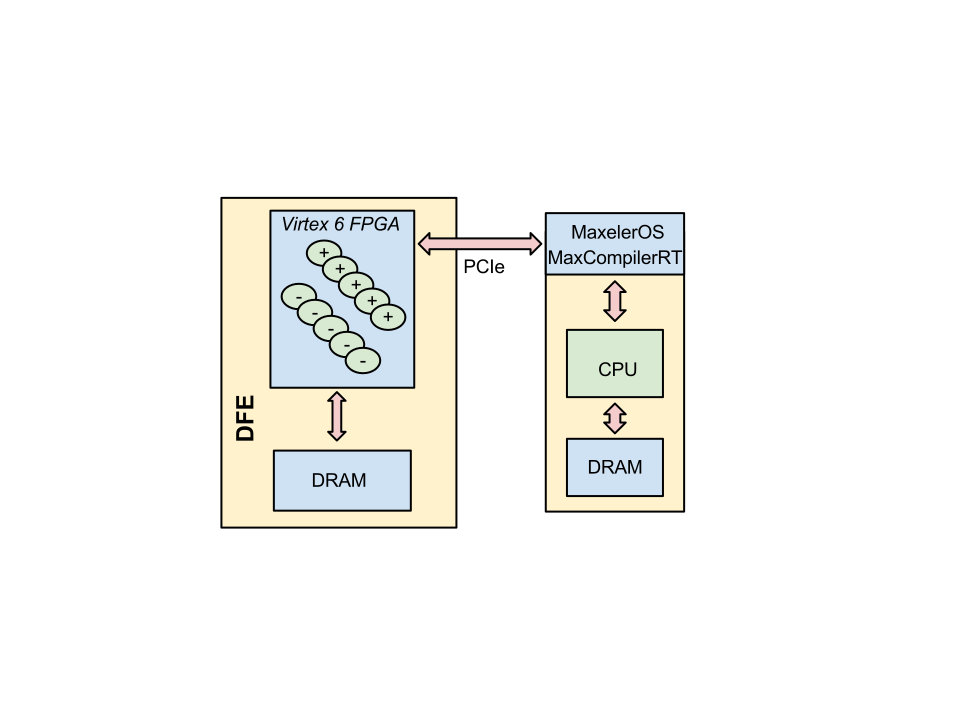
\includegraphics[scale=0.4, trim=0 200 0 200]{figs/max3.png} \caption{
The Maxeler acceleration solution: the DFE is connected to
the host machine via PCIe. The board comprises 48GB of DRAM and a
Virtex 6 FPGA chip. }
\label{fig:max3}
\end{figure}

\subsection{MaxJ}

\subsection{MaxCompiler}

MaxCompiler is a high level compiler targeting the acceleration
platform developed by Maxeler Technologies [@maxwhite]. It provides a
Java based API for specifying hardware designs that are compiled and
uploaded onto the DFE and a C runtime interface (MaxCompilerRT and
MaxelerOS shown in Figure \ref{fig:max3}) for the part of the
application running on the CPU of the host system.

We demonstrate the use of MaxCompiler in accelerating a simple moving
average computation, starting from an original design in C shown in
Listing \ref{MovingAvg-C}. This performs a three point moving average
computation on an input array x, using 2 point averages at boundaries.

\lstset{language=C++, caption={Original three point moving average
computation in C.}, label={MovingAvg-C}}

\begin{lstlisting}

for (int i = 0; i < n; i++ ) {
   sum = x[i], divisor = 1;
   if ( i > 0 )
     sum += x[i - 1], divisor++;
   if (i < n - 1)
     sum += x[i + 1], divisor++;
   y[i] = sum / divisor;
}
\end{lstlisting}



Transforming this code to use the Maxeler acceleration platform
requires us to write three programs.

First we must create a kernel design. This is written in Java and
specifies the computational datapath. Listing \ref{MovingAvg-Kernel}
shows some of the important features of the MaxCompiler API:


\begin{itemize}

\item kernel inputs and outputs provide an I/O interface that allow the
  kernel to communicate with the rest of the design (Lines 4 and 15);

\item stream offset expressions allow accessing past and future elements
  of a stream (Lines 5 and 6). The offset window is stored into on
  chip BRAM so is limited to a few tens of thousands elements;

\item frequently used components such as counters are provided by the
  API. They are useful in keeping track of iteration count when
  mapping loops to streaming designs (Line 7);

\item operator overloading is used to perform arithmetic on input streams;

\item multiplexers (in this instance represented by the overloaded
  conditional operator) are used to select between streams (Lines 11
  and 12).

\end{itemize}

All these features will have to be supported by our MaxC language as
described in Section \ref{maxc}.

\lstset{language=Java, label={MovingAvg-Kernel}, caption={Kernel
design for the three point moving average computation showing features
such as stream offsets, arithmetic and control which will have to be
supported by our MaxC language}}

\begin{lstlisting}
public class MAKernel extends Kernel{
  public MAKernel(KernelParameters parameters) {
    super(parameters);
    HWVar x = io.input("x", flt );
    HWVar x prev = stream.offset(x, -1);
    HWVar x next = stream.offset(x, +1);
    HWVar cnt = control.count.simpleCounter(32, N);
    HWVar sel nl = cnt > 0;
    HWVar sel nh = cnt < (N - 1);
    HWVar sel m = sel_nl & sel nh;
    HWVar prev = sel_nl ? x prev : 0;
    HWVar next = sel_nh ? x next : 0;
    HWVar divisor = sel_m ? 3.0 : 2.0;
    HWVar y = (prev+x+next)/divisor;
    io.output("y" , y, hwFloat(8, 24) );
  }
}
\end{lstlisting}


Next we create a manager design, also written in Java; this is used to
manage kernel I/O, connecting multiple kernels together (in multi
kernel designs) and kernels to DRAM and the CPU interface (via
PCIe). Listing \ref{MovingAvg-Manager} shows a simple design for the
moving average application that instantiates a single moving average
kernel and connects its inputs and outputs to the host interface.

\lstset{label={MovingAvg-Manager}, caption={Manager design for the
three point moving average computation}}

\begin{lstlisting}
public class MAManager extends CustomManager {
  public MAManager(MAXBoardModel board_model, boolean is_simulation, String name) {
    super(board_model, is_simulation, name);

    KernelParameters params = manager.makeKernelParameters("MAKernel");
    KernelBlock k = addKernel(new MovingAverageKernel(params));

    k.getInput("x") <== addStreamFromHost("x");
    addStreamToHost("y") <== k.getOutput("y");

  }
}
\end{lstlisting}

In Section \ref{maxcconf} we introduce a simple language to capture
this flow configuration.

Finally we must write a host application which is required to queue
the input streams and run the accelerator. This is achieved by calls
to the MaxCompilerRT (runtime) API that interfaces with MaxelerOS.

\lstset{label={MovingAverage-Host}, caption={Host example for queueing
the input and output streams and running the three point moving
average design.}}

\begin{lstlisting}
max_run(
  device,
  max_input("x", x, x_size),
  max_output("y", y, y_size),
  max_runfor("MAKernel", n),
  max_end());
\end{lstlisting}


Although the MaxCompiler toolchain greatly simplifies the process of
accelerating applications and particularly the designing of dataflow
kernels, the acceleration process is still very involved and requires
a large amount of experience with FPGA technology and domain specific
knowledge. Most importantly the whole process is manually driven
including the exploration of optimizations. This step is a critical
and time consuming part of the design process which is vital in
achieving maximum performance (in terms of operating frequency, number
of parallel pipelines etc.) subject to physical limitations such as
chip size or timing constraints.

By specifying the design in MaxC and optimization strategies in LARA
we aim to create the basis of a design space exploration flow that can
automate this process.

\subsection{Dataflow Engines}

\section{Aspect Oriented Programming}

\subsection{AspectJ}

\subsection{AspectC++}

\subsection{LARA}

Lara is an aspect oriented programming language for specifying
compiler strategies for FPGA-based systems
[@Lara1; @Lara2; @Lara3]. The key feature of LARA is that it separates
the application code from the strategies required to compile and
optimize it for a particular platform. It enables the capturing of
strategies for:

\begin{itemize}
\item instrumentation, monitoring and hardware-software partitioning
  [@Lara2]- these will be used in the initial stages of our proposed
  design flow to identify optimization candidates for mapping onto
  the accelerator

\item code specialization and code optimization [@Lara2] -- these will be
  used both for the original source code application which is the
  target of the compilation and for the dataflow design
\end{itemize}

Furthermore LARA descriptions can be parametrized which facilitates
integration with our proposed DSE step described in Section
\ref{designflow}.

Listing \ref{lara} shows an example description used for fully
unrolling all innermost loops with an iteration count smaller than or
equal to 16. The `select` statement on line 2 captures the join points
on which the aspect acts, the `apply` statement specifies actions to
be applied to the results of a query while `condition` is used to
filter relevant queries.

\lstset{style=lara, label={lara}, caption={Example LARA description
for fully unrolling innermost loops with an iteration count smaller
than or equal to 16.}}

\begin{lstlisting}
aspectdef loopunroll
  select function.loop{type="for"} end
  apply optimize("loopunroll", "fully"); end
  condition $loop.is_innermost && $loop.num_iter<=16; end
end
\end{lstlisting}

[@Lara2] also introduces a design flow based on LARA for mapping
applications into heterogeneous multicore platforms. This involves
specifying optimizations and mapping strategies in the LARA
programming language, separate from the application source code.

The strategies are compiled and applied to the original source code in
a sequential order to obtain the final design which is synthesized
using Catapult-C [@catapultc]. Examples of strategies which are
expressed using LARA include loop unrolling, coalescing, loop fission
and mapping compute intensive functions to hardware (hardware/software
partitioning).

Advantages of the aspect based approach compared with the popular
pragma based approach used in frameworks like OpenMP [@openmppragma]
include the possibility of defining dynamic join points through which
strategies can be applied to the intermediate results of the weaving
(source translation) process. Additionally optimization strategies are
grouped into cohesive aspects, rather than being spread through the
code which makes them easier to understand, maintain and modify, for
example to target a different platform.


\section{Related Work}

\subsection{High Level Synthesis}

Substantial work has been carried out in synthesizing high level
languages to hardware designs and many tools exist for this purpose
[@ctoverilog; @vivadodesignsuite; @impulsec]. However most approaches
do not target a streaming dataflow architecture but either soft
processor designs - processor cores implemented on the FPGA chip with
configurable custom computing units (e.g. floating point units). These
usually offer limited speedups when compared to high-end hardcore
CPUs but can turn out to be more energy efficient.


[@stancl] proposes a method for synthesising hardware pipelines from
OpenCL programs which exploits some important concepts related to
parallelism exposed by the OpenCL specification [@opencl] such as
threads and domain decomposition into threads sharing local memory.
Although we are dealing with simple C kernels for this project, some
of the proposed compilation strategies can be applied for
loop.

\subsection{Dataflow Languages}
A number of dataflow languages have been developed targeting FPGAs but
also multi-core platforms. Table \ref{table:feature-comparison}
summarises some of the important features of these languages compared
to \FAST{}.

Lucid \cite{ashcroft1977lucid}, SISAL \cite{gurd1987implicit},
\cite{mcgraw1983sisal} and Lustre \cite{halbwachs1991synchronous}, are
examples of functional dataflow languages. The latter is based on a
synchronous programming model, facilitating safety verification for
critical software \cite{halbwachs1992programming} rather than
performance. The functional programming style complicates the
translation of existing imperative applications and none have existing
implementations for FPGAs, so a performance comparison is not
possible.

Streams-C\cite{Gokhale:Stone:Arnold:Kalinowski:2000} and
ImpulseC\cite{ImpulseC} adopt imperative ANSI C syntax and an
execution model based on Communicating Sequential Processes and
introduce non-standard syntax and constructs for specifying designs
such as special comment blocks which are used to annotate the C
application code. The specialised syntax makes the languages harder to
integrate with existing source-to-source translation or aspect weaving
frameworks.

Hybrid approaches such as MaxCompiler\cite{5719584} separate the CPU
run-time component from the accelerated one, providing a C run-time
environment and a Java API for building dataflow designs via
meta-programming. The separation complicates the development process,
hindering sharing of design parameters and, consequently, the design
space exploration process. The use of meta-programming simplifies
design parametrisation, but can make resulting programs harder to
understand. In contrast, the proposed approach allows the computation
description, which includes CPU and dataflow components, to be specified
using a single language and to be decoupled from design
parametrisation and other optimisation strategies which are captured
as LARA aspects. This separation of concerns results in more intuitive
and maintainable descriptions.

\begin{sidewaystable}[!ht]
  \renewcommand{\arraystretch}{2.1}
  \centering
  \label{table:feature-comparison}
  \begin{tabularx}{\textwidth}{ m{2.5cm} | p{2.5cm} | p{3cm} | p{1.9cm}| p{2.8cm} | p{3.2cm} | p{2.5cm}}
    \hline
    \bf{Language}                 & \bf{Syntax}              & \bf{Paradigm}                            & \bf{Support}              & \bf{Implementation}             & \bf{Design Parametrisation}                     & \bf{Optimisation Strategies}            \\
    \hline \hline
    \bf{Lucid}                    & Lucid                    & Functional                               & \multirow{3}{*}{Software} & \multirow{3}{*}{Multiprocessor} & \multirow{3}{3cm}{Manual Source Transformation} & \multirow{5}{3cm}{Manual Code Revision} \\
    \cline{1-3}
    \bf{SISAL}                    & SISAL                    & Functional                               &                           &                                 &                                                 &                                         \\
    \cline{1-3}
    \bf{Lustre}                   & Lustre                   & Synchronous                              &                           &                                 &                                                 &                                         \\
    \cline{1-6}
    \bf{MaxCompiler}              & C99(SW) Java(HW)         & Imperative(SW) Dataflow(HW)              & \multirow{6}{*}{Combined} & \multirow{6}{*}{CPU + FPGA}     & Meta-programming                                &                                         \\
    \cline{1-3}\cline{6}
    \bf{Streams-C} \bf{ImpulseC}\ & C99                      & Imperative(SW) CSP(HW)                   &                           &                                 & Compiler \newline Directives                    &                                         \\
     \cline{1-3}\cline{6-7}
    \bf{\FAST{}}/\bf{LARA}        & C99(SW/HW) LARA(Aspects) & Imperative(SW) Dataflow(HW) AOP(Aspects) &                           &                                 & \multicolumn{2}{p{5.5cm}}{Compiler Directives + \newline Automated Aspect-Directed Source Transformation} \\
  \end{tabularx}
  \caption{Feature comparison of the \FAST{}/LARA approach and existing dataflow implementations.}
\end{sidewaystable}


\subsection{Aspect-driven Compilation of FPGA Designs}

One attempt at capturing optimisation strategies for FPGA designs
 using aspect descriptions is LARA
 \cite{Cardoso:Carvalho:Cutinho:Luk:Nobre:Diniz:Petrov:2012,
   Cardoso:Carvalho:Teixeira:Diniz:Goncalves:Petrov:2012}, an Aspect
 Oriented language for embedded systems. Aspect descriptions are
 written in the LARA language and automatically applied to the
 original application source to generate optimised versions through
 various transformations that enable and optimise hardware/software
 partitioning \cite{Lam:Coutinho:Luk:2008}. Aspect descriptions can be
 used to specify compilation strategies that result in overall
 speedups of 2 to 6.8 times over software versions
 \cite{Cardoso:Teixeira:Alves:Nobre:Diniz:Cutinho:Luk:2012}, generally
 with high aspect bloat \footnote{ $\text{aspect bloat} =
   \frac{\text{size of transformed code}}{\text{size of original
       code}}$, so a higher aspect bloat is better}
 \cite{Cardoso:Carvalho:Cutinho:Luk:Nobre:Diniz:Petrov:2012}.

The use of LARA aspects in guiding the compilation process of C
applications is described in
\cite{Cardoso:Teixeira:Alves:Nobre:Diniz:Cutinho:Luk:2012} and
\cite{cardoso2011new} but the backend compilation targets a von
Neumann architecture (with a GPP and custom accelerator) unlike the
dataflow architecture proposed in this paper. The approach described
in \cite{Cardoso:Teixeira:Alves:Nobre:Diniz:Cutinho:Luk:2012} and
\cite{cardoso2011new} relies more on high-level source transformation
whereas our approach is based on a systematic design space exploration
process, which enables the analysis of more low-level
optimisations. Finally,
\cite{Cardoso:Teixeira:Alves:Nobre:Diniz:Cutinho:Luk:2012} and
\cite{cardoso2011new} do not consider development aspects which can be
used to improve developer productivity.


The use of aspect-oriented programming for specifying strategies for
run-time adaptation of FPGA designs discussed in \cite{6322875}
differs from the static process considered in this paper in which the
application is partitioned and scheduled at compile time, to achieve
optimised performance as described in
\cite{Xinyu:Qiwei:Luk:Qiang:Pell:2012}. An advantage of our approach
is that an optimised allocation is generated prior to application
execution. However, we lack the flexibility of adapting the design to
varying input conditions.

\section{Summary}

\section{Design Flow}
\label{sec:design-flow}

To improve both efficiency and productivity, our design flow focuses
on maintaining or improving the \emph{performance} and \emph{energy
  efficiency} of existing applications while using a more systematic
approach for design optimisation that results in more \emph{portable}
application code, improves \emph{integration} with existing
applications and \emph{automates} manual, time consuming and
error-prone tasks.

\begin{comment}
Our design flow aims to improve both \emph{efficiency} (in terms of
performance and energy consumption) and \emph{productivity}. The
former is crucial to High Performance Computing, the latter helps
reduce development cost and time and is a well-known issue with
existing FPGA based acceleration solutions \cite{jones2010gpu}. To
achieve this we focus on maintaining or improving the
\emph{performance} and \emph{energy efficiency} of existing
applications while using a more systematic approach for design
optimisation that results in more \emph{portable} application code,
improves \emph{integration} with existing applications and
\emph{automates} manual, time consuming and error-prone tasks.
\end{comment}

The key components of the design flow are:
\begin{itemize}
\item \emph{\FAST{}}, a novel language for specifying dataflow designs
  which is compatible with C syntax, improving developer productivity
  and supporting combined hardware and software specifications;

\item \emph{aspect driven compilation flow}, used to decouple
  optimisation from design development, improving design portability,
  and automating the generation of code and design space
  exploration~\footnote{the process of exploring multiple
    configurations to identify optimal implementations} which improves
  productivity;

\item \emph{systematic design space exploration}, to identify maximum
  performance configurations by using \emph{aspect descriptions} to
  conveniently control and guide the exploration process based on
  user-specified constraints;
\end{itemize}

\Cref{fig:design-flow} illustrates the design flow:
\begin{enumerate}
\item a C application containing an embedded high-level dataflow
  design specified in \FAST{} is developed from the original source
  application;
\item the dataflow design is transformed by the aspects in the
  repository to generate new configurations (e.g. with multiple
  word-length configurations);
\item the generated configurations are compiled using a backend
  compilation toolchain (MaxCompiler) to dataflow designs
  implemented on FPGAs;
\item the feedback from the compilation process is used to drive
  design space exploration, repeating the weaving and compilation
  process until user-specified constraints are satisfied.
\end{enumerate}

\begin{figure}[!ht]
  \centering
  \def\svgwidth{0.8\linewidth}
  \input{figs/asap13-design-flow.pdf_tex}
  \caption{Proposed approach for aspect-driven compilation of dataflow
   designs.}
  \label{fig:design-flow}
\end{figure}
\section{FAST}

\begin{frame}[fragile]
  \frametitle{2. FAST -- Facile Aspect-driven Source Transformation}

\begin{lstlisting}
void Price_FPGA(float* stockPrices, float* result,
                float c1, float c2, float c3,
                int nStocks, int order, int timesteps) {
  int step  = (CURRENT_CYCLE / n1) \% timesteps;

  #pragma fast DSPBalance:full
  float inter =  stockPrices[0] * c1
       + stockPrices[1] * c2 + stockPrices[-1] * c3;
  bool up = (step >= order) && (step < nStocks - order);
  result[0] = up ? inter : stockPrices);
}

void Price_CPU(...) { /* Regular C implementation */}

int main() {
  #pragma fast hw:Price_FPGA
  Price_CPU(...);
}
\end{lstlisting}
\end{frame}

\begin{frame}
  \frametitle{2. FAST: Features}

\begin{table}[!h]
  \centering
\renewcommand{\arraystretch}{1.4}
\begin{tabular}{l|l|l}
\hline
\bf{Feature}                        & \bf{Description}              & \bf{Method}          \\
\hline\hline
  I/O                               & Kernel arguments              & Inferred             \\
\hline
  Control                           & Ternary op. (?:), \texttt{if} & C99                  \\
\hline
\multirow{2}{*}{Computation}        & +, *, /, -                    & C99                  \\
                                    & log, exp, sqrt, sin etc.      & $<$math.h$>$         \\
\hline
  \multirow{2}{*}{Streams}          & Declared as pointers          & \multirow{2}{*}{C99} \\
                                    & Array index access     &                      \\
\hline
  Optimisation                      & \multirow{2}{*}{C pragmas}    & \multirow{2}{*}{C99} \\
  Hardware \  Mapping               &                               &                      \\
\hline
  \multirow{2}{*}{Parameterization} & Constants, variables,         & \multirow{2}{*}{C99} \\
                                    & \texttt{for}, \texttt{while}  &                      \\
\end{tabular}
\end{table}
\end{frame}

\begin{frame}{2. FAST: FAST vs C}
\begin{itemize}
\item Fast only uses C syntax to simplify integration with compiler
  frameworks.
\item  Key differences
\begin{itemize}
\item execution model only supports kernels
\item pointers are regarded as   streams
\item negative offsets are allowed
\item only compile time loop bounds are allowed
\item direct interoperability with C code is not possible, but
  simulated via pragmas
\end{itemize}
\end{itemize}

\end{frame}
\section{Aspect Descriptions}
\begin{frame}
  \frametitle{Aspect Descriptions}
\begin{enumerate}
  \item  system aspect descriptions (e.g. monitor performance)
  \item implementation aspect descriptions (e.g. optimise word-length for operators)
  \item exploration aspect descriptions (e.g. control automation of design space exploration)
  \item development aspect descriptions (e.g. assist debugging)
\end{enumerate}

\end{frame}


\begin{frame}
  \frametitle{System Aspects}
Hardware/Software Partitioning:
\begin{enumerate}
  \item detect hotspots
  \item detect code patterns suitable for acceleration
  \item perform outlining transformation
  \item derive dataflow \texttt{fast\_f()} from \texttt{f()}
  \item place FAST pragma to link \texttt{fast\_f()} with \texttt{f()}
\end{enumerate}
\end{frame}


\begin{frame}[fragile]
  \frametitle{System Aspects: Monitoring}
  For all innermost loops:
\begin{itemize}
  \item Monitor every loop iteration
  \item Monitor every loop entry and exit
\end{itemize}
\begin{lstlisting}[label=lst:label, style=lara]
aspectdef LoopMonitor
  function.loop{is_innermost}:
    entry:   prepend(mon_iterationIn());
    exit :   append (mon_iterationOut());
    default: prepend(mon_instanceIn());
             append(mon_instanceOut());
end
\end{lstlisting}
\end{frame}

\begin{frame}
  \frametitle{Monitorisation: Aspect Weaving}
\begin{center}
\renewcommand{\arraystretch}{1.2}
\begin{tabular}{p{5cm}|p{5cm}}
\hline
\bf{Original Code}           & \bf{Woven Code}                                   \\
\hline
void f() \{                  & void f() \{                                       \\
                             & \hspace{3ex}\emph{monitor\_instanceI("f:1");} \\
\hspace{3ex}while (i $ < $ N) \{ & \hspace{3ex}while (i$ < $N) \{                      \\
                             & \hspace{6ex}\emph{monitor\_iterI("f:1");}     \\
\hspace{6ex}i++;             & \hspace{6ex}i++;                                  \\
                             & \hspace{6ex}\emph{monitor\_iterE("f:1");}     \\
\hspace{3ex}\}               & \hspace{3ex}\}                                    \\
                             & \hspace{3ex}\emph{monitor\_instanceE("f:1");} \\
\}                           & \}                                                \\
\end{tabular}
\end{center}
\end{frame}

\begin{frame}{System Aspects: Run-time Reconfiguration}
Explain why run-time reconfiguration is useful
\end{frame}

\begin{frame}{System Aspects: Run-time Reconfiguration}
Show aspects for run-time reconfiguration and general strategy
\end{frame}

\begin{frame}[fragile]{Implementation Aspects: Operator Optimisation}
\begin{lstlisting}[label=lst:label, style=lara]
aspectdef DspBalancing
var op_granularity =
 [{DspBalance:’full’,MultiplyOp: 5,AddOp: 5 },
  {DspBalance:’balanced’,MultiplyOp:3}];

select function.statement end
apply
 for (var i in op_granularity) {
   var gprofile = op_granularity[i];
   var match = true;
   for (var k in gprofile) {
     if (k != ’DspBalance’) {
       match &= ($statement.num_construct(k)
                 >= gprofile[k]);}}
   if (match) {
     var pragma = ’#pragma FAST balanceDSP:’
                   + gprofile.DspFactor;
     $statement.insert before "[[pragma]]";
     break;}}
   end
end
\end{lstlisting}
\end{frame}

\begin{frame}[fragile]{Exploration Aspects: Control DSE}
\begin{lstlisting}[label=lst:label, style=lara]
aspectdef DesignExploration
  input
   attribute,
   start, step,
   resource, resource_threshold,
   config
end
config[attribute] = start;
var i = 0;
do {
  var designName = genName(config);
  call genFAST(designName, config);
  buildFAST(designName);
  config[attribute] += step; i++;
} while (@hw[designName]. resource < resource_threshold && i < LIMIT);
end
\end{lstlisting}
\end{frame}

\begin{frame}[fragile]{Development Aspects: Debugging}
\begin{lstlisting}[label=lst:label, style=lara]
aspectdef WatchVar
select function.vref end
apply
  $vref.parent_stmt.insert before
  %{ log("[[$vref.name]]", [[$vref.name]]); }%
  $vref.parent_stmt.insert after
  %{ log("[[$vref.name]]", [[$vref.name]]); }%
end
condition $vref.is_out end
end
\end{lstlisting}

\begin{itemize}
\item useful since no run-time is debugger available
\item aspect descriptions automatically log values of variables on assignment
\end{itemize}
\end{frame}

\section{Evaluation}

\subsection{RTM Implementation}
We evaluate the proposed approach by implementing a high-performance
application based on the Reverse Time Migration method for seismic
imaging which is used to detect geological structures, based on the
Earth's response to injected acoustic waves. The technique models the
propagation of injected waves using the isotropic acoustic wave
equation \cite{araya2011assessing}:
\begin{align}
\frac{d^2p(r,t)}{dt^2} + {dvv(r)}^2\bigtriangledown^2p(r,t) = f(r,t)
\end{align}
We approximate the differential equation using stencil computation to
perform a fifth-order Taylor expansion in space and first-order Taylor
expansion in time.

We use MaxC to implement the dataflow kernels and aspects to generate
multiple configurations for the design by creating two kernels that
are used to control the memory command read and write streams
(CmdRead, CmdWrite) and the computation kernel (RTM).  To illustrate
the potential benefits of our approach we analyse the results of using
the debugging aspect of Section \ref{sect:asp_debug}. Table
\ref{table:loc} compares the number of lines of code required for the
original MaxC + Aspect implementation with the equivalent MaxJ
implementation showing a reduction in code size of up to 42\% for the
run-time reconfigurable design and a reduction in the number of API
calls (including debug calls) of up to 67\% which translate to
increase productivity.

\begin{table}[!h]
  \renewcommand{\arraystretch}{1.3}
  \centering
  \caption{Code measures for the RTM kernels comparing MaxC and
    MaxJ.}
  \label{table:loc}
  \begin{tabular}{c|ccc|cc}
    \hline
    \multirow{2}{*}{\bf{Kernel}} & \bf{Aspect } & \multicolumn{2}{c|}{\bf{MaxC}} & \multicolumn{2}{c}{\bf{MaxJ}}                   \\
    \                            & \bf{LOC}     & \bf{LOC}                       & \bf{\# API calls} & \bf{LOC} & \bf{\#API Calls} \\
    \hline \hline
    CmdRead                      & 12           & 26                             &      6         & 59       &      39        \\
    CmdWrite                     & 12           & 28                             &      39        & 79      &       56         \\
    RTM Static                   & 12           & 246                            &     43         & 403     &       175        \\
    RTM RTR                      & 12           & 377                            &     91         & 669     &       275       \\
  \end{tabular}
  \vspace{-3mm}
\end{table}

\subsection{Results}

Results of the design space exploration using the aspect in
Fig.~\ref{fig:aspect-exploration} with variable mantissa illustrate
the trade-offs between accuracy and resource usage
(Fig.~\ref{fig:precision}). We observe irregular, large variations
when decreasing the mantissa from 18 to 16 and 24 to 22. This is the
effect of the backend tools mapping arithmetic to a combination of
both DSPs and LUT/FF elements. The mantissa boundaries at which this
optimisation occurs are platform specific, depending on the
architecture of the DSPs. Hence automating this optimisation via
aspects and decoupling it from the original source code makes the
application more portable and facilitates discovery of interesting
trade-off opportunities using design space exploration.

\begin{figure}[!h]
\includegraphics[scale=0.7]{figs/pre}
\caption{Exploration of accuracy vs resource usage trade-offs using the aspect
shown in Fig.~\ref{fig:aspect-exploration} with variable mantissa.}
\label{fig:precision}
  \vspace{-2mm}
\end{figure}

The DSP balancing aspect shown in Fig.~\ref{fig:aspect-DSP} allows to
explore the resource trade-offs of implementing arithmetic operations
in either DSPs or LUTs and FFs (Fig.~\ref{fig:arith}). This helps to
avoid over mapping on DSPs for arithmetic intensive applications.

\begin{figure}[!h]
\includegraphics[scale=0.7]{figs/arith}
\caption{Exploration of DSP and LUT/FF balancing for arithmetic
  operations using the aspect shown in Fig.~\ref{fig:aspect-DSP}.}
\label{fig:arith}
  \vspace{-2mm}
\end{figure}

Design space exploration using the aspect in
Fig.~\ref{fig:aspect-exploration} with increasing parallelism level
can be used to investigate design scalability. For example for the
described RTM implementation, Fig.~\ref{fig:scalability} shows that
performance scales linearly with the number of parallel
pipelines. This also shows that significant speedups can be obtained
by the MaxC dataflow design compared to the CPU only
implementation. Depending on the problem size, our approach can be
used to achieve a significant speedup over software only versions
which is comparable with the best published FPGA results for static
designs \cite{Xinyu:Qiwei:Luk:Qiang:Pell:2012},
\cite{araya2011assessing}.

\pgfplotsset{every axis x label/.style={
  at={(0.5,0)},
  below,
  yshift=-5pt}}

\pgfplotsset{every axis y label/.style={
  at={(0,0.5)},
  xshift=-20pt,
  rotate=90}}

\begin{figure}[!h]
  \centering
  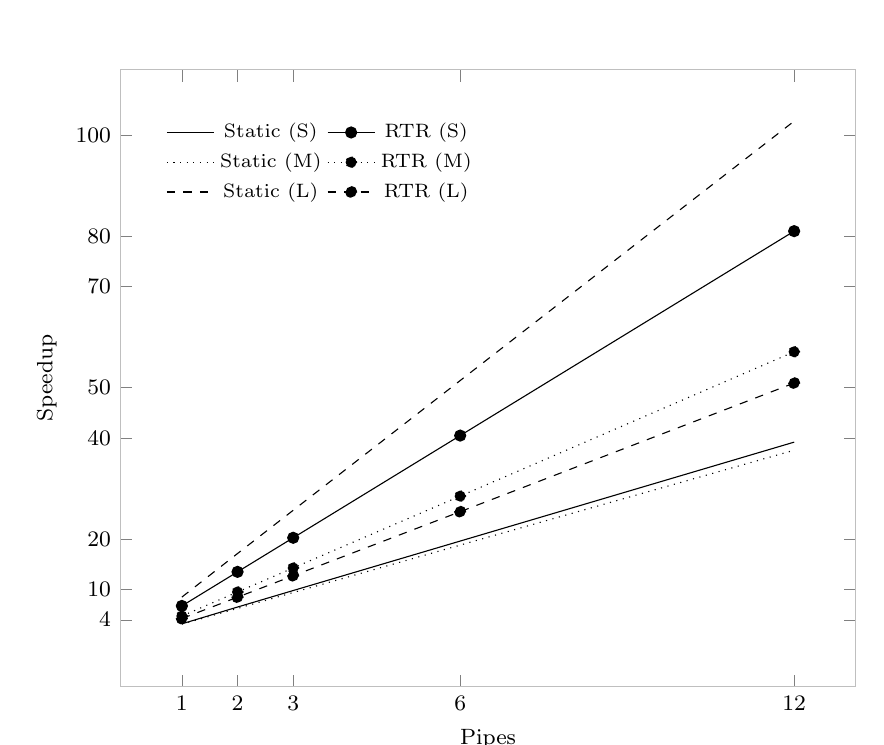
\begin{tikzpicture}
    \selectcolormodel{gray}
    \begin{axis}[
        xmin=1,
        ymin=1,
        %no markers,
        font=\tiny,
        xlabel=Pipes,
        ylabel=Speedup,
        xtick={1,2,3,6,12},
        ytick={4, 10, 20, 40, 50, 70, 80, 100},
        legend columns=2,
        legend entries={
          Static (S),
          RTR (S),
          Static (M),
          RTR (M),
          Static (L),
          RTR (L)},
        legend style={
          draw=none,
          at={(0.05,0.85) },
          anchor=west
        }
      ]

      \addplot[mark=none] coordinates {
        (1, 3.2)
        (2, 6.53)
        (3, 9.8)
        (6, 19.6)
        (12, 39.2)
      };
      \addplot[mark=*] coordinates {
        (1, 6.75)
        (2, 13.5)
        (3, 20.25)
        (6, 40.5)
        (12, 81)
      };
      \addplot[dotted] coordinates {
        (1, 3.13)
        (2, 6.26)
        (3, 9.4)
        (6, 18.8)
        (12, 37.6)
      };
      \addplot[mark=*, dotted] coordinates {
        (1, 4.75)
        (2, 9.51)
        (3, 14.27)
        (6, 28.5)
        (12, 57.1)
      };
      \addplot[mark=none, dashed] coordinates {
        (1, 8.5)
        (2, 17.13)
        (3, 25.7)
        (6, 51.4)
        (12, 102.8)
      };
      \addplot[mark=*, dashed] coordinates {
        (1, 4.25)
        (2, 8.48)
        (3, 12.725)
        (6, 25.42)
        (12, 50.9)
      };2
    \end{axis}
  \end{tikzpicture}
  \caption{Scalability of the RTM dataflow design explored using the aspect
shown in Fig.~\ref{fig:aspect-exploration}.}
  \label{fig:scalability}
  \vspace{-2mm}
\end{figure}

Fig.~\ref{fig:scalability} also shows the performance benefits of
using a run-time reconfiguration implementation which is generated by
using the reconfiguration aspect of Fig. 4 to create two
configurations for the RTM MaxC kernel. Since during the first half of
the execution the backward propagation and imaging functions are idle,
the first configuration requires only half the resources. This allows
doubling the number of parallel pipelines and halves the execution
time of the first configuration. The speedup obtained is comparable to
\cite{Xinyu:Qiwei:Luk:Qiang:Pell:2012}, but the partitioning and
optimisation exploration process is automated via aspects, which
increases developer productivity. The automated process improves
portability of the design, allowing optimisations based on design
space exploration to be carried out on various platforms (hence
subject to varying resource constraints) without manual intervention.

\section{Conclusion}

In this paper we present an automated design flow for design space
exploration of dataflow designs based on a novel language, MaxC, and
aspect-driven compilation. We show that this approach meets the
initial performance, portability, integration and productivity
requirements. We implement a high performance dataflow design for RTM
to show that we can achieve significant speedups over software only
versions by exploiting the run-time reconfiguration. The automated
aspect-driven optimisation process improves productivity and design
portability, allowing optimisations strategies to be automatically
adapted to various platforms.  Finally we show that MaxC is a concise
language and that maintaining compatibility with C99 simplifies the
translation of existing applications.

Future work includes extending our approach by introducing new system
aspects that guide the translation and optimisation process from
existing C applications to dataflow designs. This includes the
development of system aspects that can be used to explore structural
transformations of the original application that improve parallelism
and computation versus communication ratio. The introduction of these
aspects could lead to a transparent design flow, that does not require
manual development of dataflow designs, greatly simplifying the
translation of existing software applications to high-performance
custom designs.



% some spacing
\newcommand{\BIBdecl}{\setlength{\itemsep}{0.4 em}}

\bibliographystyle{IEEEtran}
\bibliography{../../refdb/bibliography.bib}

\clearpage
\appendix

\chapter{User Guide}

\fastc{} is an experimental compiler for the \FAST{} language and is
available at \url{https://github.com/paul-g/maxcc}.

\section*{Installation}

The project requires \footnote{Please check the documentation of these
  tools for other dependencies.}: \emph{1)} GNU AutoTools
\cite{Autotools}, \emph{2)} Boost 1.47\cite{boost1.47} and \emph{3)}
ROSE 0.9.5 \cite{ROSE}. To extract and compile the project please run
the following commands:

\begin{lstlisting}
tar xvzf fastc-${version}.tar.gz && cd fastc-${version}
configure --with-boost=/path/to/boost --with-rose=/path/to/rose
make && make install
\end{lstlisting}

\section*{Testing}

To test your installation run \texttt{make test}.

\section*{Where To Start}

Please visit the \FAST{} wiki at https://github.com/paul-g/maxcc/wiki
to get started.

\input{sections/RTM-original.tex}
\chapter{Original Memory Read Kernel}
\label{app:mem-read-kernel}
The following listing shows the original memory read kernel for the
Reverse Time Migration application implemented with MaxJ using
MaxCompiler 2012.1. This kernel generates the memory commands required
to fetch data from DRAM. Some typical Java constructs such as package
definitions and imports are omitted.
\begin{lstlisting}
public class Cmdread extends Kernel {
    public Cmdread(..) {
      int   Burst_inc     =1;
      HWVar iniBursts     =io.scalarInput("iniBursts",hwUInt(32));
      HWVar totalBursts   =io.scalarInput("totalBursts",hwUInt(32));
      HWVar wordsPerBurst =io.scalarInput("wordsPerBurst",hwUInt(32));
      HWVar Enable        =io.scalarInput("Enable",hwUInt(1));

      //the address counters
      Count.Params param0 = control.count.makeParams(32)
           .withEnable(Enable).withMax(wordsPerBurst).withInc(1);
      Counter counter0    = control.count.makeCounter(param0);
      HWVar  wordCount    = counter0.getCount();
      Count.Params param1 = control.count.makeParams(32)
           .withEnable(counter0.getWrap()).withMax(totalBursts).withInc(Burst_inc);
      Counter counter1    = control.count.makeCounter(param1);
      HWVar burstCount    = counter1.getCount();
      HWVar Control       = wordCount.eq(0) & Enable;
      DRAMCommandStream.makeKernelOutput("dram_read", (*@\label{app:memrk-dram}@*)
          Control,                          // control
          burstCount+iniBursts,             // address
          constant.var(hwUInt(8),Burst_inc),// size
          constant.var(hwUInt(6),  1),      // inc
          constant.var(hwUInt(4),  0),      // stream
          constant.var(false));

    }}
\end{lstlisting}
\chapter{FAST Dataflow Kernels}

\section{Numerical Differentiation}

The \FAST{} dataflow kernel that implements the differentiation
operation is shown in Listing {}. It uses no API (non-user defined)
function calls and a total of 20 lines of code.

\begin{lstlisting}
#include ``fastc/fast.h''

const int Par;

int stream_diff(float *value[Par], int offset, int pipe) {
  int cycle_offset = (pipe + offset) / Par;
  int pipe_offset  = (pipe + offset) % Par;

  int cycle_offset_neg = (Par - 1 - pipe + offset) / Par;
  int pipe_offset_neg  = Par - 1 - (Par - 1 - pipe + offset) % Par;
  return value[pipe_offset][cycle_offset] -
         value[pipe_offset_neg][cycle_offset_neg];
}

int diff(float *value[Par], float h, int pipe) {
  return (-2 * stream_diff(value, 2, pipe)
          -1 * stream_diff(value, 1, pipe)) / (10 * h);
}

void kernel_SGDiff( float* value[Par], int width, int size, double step){
  int cycle = Par * CYCLE_COUNT + pipe;
  bool compute = (cycle >= width) & (cycle < size - width);

  for (int pipe = 0; pipe < Par; pipe++) {
    result[pipe] = compute ? diff(value, h, pipe) : value[pipe]
  }
}
\end{lstlisting}

\section{Add Prediction}
\chapter{Experimental Data}
\label{app:experimental-data}

This chapter contains experimental data for the application benchmarks
that were omitted from the main report body for the sake of brevity.

Design space exploration results for the Reverse Time Migration
application are shown in \Cref{table:rtm-dse}

Experimental speedup results for our implementation of the bitonic
sorting network design are listed in \Cref{table:bit-data}.

  \begin{sidewaystable}
    \renewcommand{\arraystretch}{1.3}
    \begin{tabularx}{\textheight}{p{3.5cm}|X|X|X|X|X|X|X|X|X|X|X|X|p{1cm}|}
      \textbf{Aspects} & \textbf{DSP Balance} & \textbf{Par} & \textbf{Mem Freq} & \textbf{Width} & \textbf{FPGA Time (Ms)} & \textbf{Total Time (s)} & \textbf{Total Power (Watt)} & \textbf{Dyn. Power (Watt)} & \textbf{LUT (\%)} & \textbf{FF(\%)} & \textbf{BRAM (\%)} & \textbf{DSP (\%)} & \textbf{Build Time} \\
      \hline \hline
      \multirow{5}{2cm}{OptimizeDSPUsage, ExploreParallelism}     & Bal.    & 1   & 303      & 8\_24 & 492             & 3.347          & 117                & 30                & 19.89    & 14.13  & 23.31     & 1.69     & 1h49      \\
      & None        &     &          &       & 492             & 3.453          & 117                & 30                & 22.62    & 15.56  & 23.31     & 0        & 2 h 9      \\
      & Full        &     &          &       & 492             & 3.103          & 117                & 30                & 17.68    & 12.79  & 23.31     & 5.8      & 2 h 2      \\
      \hline
      & Bal.    & 2   &          &       & 247             & 2.917          &   121                & 34                & 25.44    & 25.44  & 24.53     & 3.37     & 2h30       \\
      & None        &     &          &       & 247             & 3.006          &       121                & 34                & 30.95    & 20.53  & 24.53     & 0        & 3h5        \\
      & Full        &     &          &       & 246             & 3.153          &       121                & 34                & 21.18    & 15     & 24.44     & 11.61    & 2h8        \\
      \hline
      & Bal.    & 3   &          &       & 225             & 3.506          & 121                & 34                & 31.56    & 21.32  & 24.06     & 5.06     & 2h30       \\
      & None        &     &          &       & 224             & 3.124          & 121                & 34                & 39.16    & 25.61  & 24.06     & 0        & 3h20       \\
      & Full        &     &          &       & 226             & 3.123          & 125                & 38                & 25.06    & 17.3   & 23.97     & 17.41    & 2h18       \\
      \hline
      & Bal.    & 6   &          &       & 226             & 3.125          & 125                & 38                & 52.61    & 30.52  & 20.12     & 17.41    & 3h17       \\
      & None        &     &          &       & 223             & 3.156          & 125                & 38                & 65.11    & 40.58  & 28.95     & 0        & 4h50       \\
      & Full        &     &          &       & 224             & 3.016          &       122                & 35                & 35.63    & 24.11  & 27.73     & 34.82    & 3h42       \\
      \hline
      \multirow{5}{2cm}{OptimizeWordWidth, OptimizeFrequency, ExploreParallelism}        & Full        & 6   & 303      & 8\_22 & 224             & 2.98           & 122                & 35                & 45.02    & 31.17  & 27.73     & 15.18    & 3h13       \\
      &             &     &          & 8\_20 & 224             & 3.006          &       122                & 35                & 43.54    & 29.96  & 27.16     & 15.18    & 3h30       \\
      &             &     &          & 8\_18 & 224             & 3.076          & 122                & 35                & 40.81    & 28.68  & 26.88     & 15.18    & 3h13       \\
      &             &     &          & 8\_16 & 224             & 3.033          & 122                & 35                & 39.62    & 26.44  & 26.6      & 10.12    & 2h50       \\
      &             &     &          & 8\_24 & 82              & 1.723          & 122                & 35                & 34.13    & 24.09  & 27.73     & 34.82    & 4h17       \\
      \hline
      &             & 2   & 400      & 8\_24 & 247             & 3.133          &       122                & 35                & 21.32    & 14.98  & 24.44     & 11.61    & 2h30       \\
      &             & 3   &          & 8\_24 & 164             & 2.964          & 122                & 35                & 25.43    & 17.28  & 23.97     & 17.41    & 2h35       \\

    \end{tabularx}
    \caption{Design space exploration results for the RTM benchmark application.}
    \label{table:rtm-dse}
  \end{sidewaystable}

\begin{table}
  \renewcommand{\arraystretch}{1.1}
  \begin{tabularx}{\textwidth}{X|X|X|X|X|X|X}
    \hline
    \textbf{Network Size}        & \textbf{log(n)}      & \textbf{CPU Time} & \textbf{FPGA Time} & \textbf{Compute Speedup} & \textbf{FPGA Total Time} & \textbf{FPGA Total Speedup} \\
    \hline \hline
    \multirow{10}{*}{128}   & 14          & 0.156162 & 0.006564  & 23.79           & 1.006564        & 0.1551             \\
    & 15          & 0.312428 & 0.013028  & 23.98           & 1.013028        & 0.3084             \\
    & 16          & 0.624328 & 0.026263  & 23.77           & 1.026263        & 0.6084             \\
    & \textbf{17} & 1.24981  & 0.051905  & 24.08           & 1.051905        & \textbf{1.1881}    \\
    & 18          & 2.49068  & 0.102083  & 24.4            & 1.102083        & 2.26               \\
    & 19          & 4.98994  & 0.199928  & 24.96           & 1.199928        & 4.1585             \\
    & 20          & 9.97521  & 0.400709  & 24.89           & 1.400709        & 7.1215             \\
    & 21          & 19.9636  & 0.807231  & 24.73           & 1.807231        & 11.0465            \\
    & 22          & 39.9202  & 1.614437  & 24.73           & 2.614437        & 15.2691            \\
    & 23          & 79.8726  & 3.203924  & 24.93           & 4.203924        & 18.9995            \\
    \hline
    \multirow{8}{*}{64} & 16          & 0.271163 & 0.012983  & 20.89           & 1.012983        & 0.2677             \\
    & 17          & 0.541016 & 0.025841  & 20.94           & 1.025841        & 0.5274             \\
    & \textbf{18} & 1.08533  & 0.052019  & 20.86           & 1.052019        & \textbf{1.0317}    \\
    & 19          & 2.16697  & 0.10265   & 21.11           & 1.10265         & 1.9652             \\
    & 20          & 4.33626  & 0.203208  & 21.34           & 1.203208        & 3.6039             \\
    & 21          & 8.66081  & 0.406241  & 21.32           & 1.406241        & 6.1588             \\
    & 22          & 17.3281  & 0.806145  & 21.5            & 1.806145        & 9.594              \\
    & 23          & 34.6705  & 1.617021  & 21.44           & 2.617021        & 13.2481            \\
    \hline
    \multirow{6}{*}{32}     & 18          & 0.458403 & 0.026085  & 17.57           & 1.026085        & 0.4467             \\
    & 19          & 0.917055 & 0.051485  & 17.81           & 1.051485        & 0.8722             \\
    & \textbf{20} & 1.83439  & 0.100844  & 18.19           & 1.100844        & \textbf{1.6663}    \\
    & 21          & 3.67453  & 0.203696  & 18.04           & 1.203696        & 3.0527             \\
    & 22          & 7.35396  & 0.404244  & 18.19           & 1.404244        & 5.237              \\
    & 23          & 14.6802  & 0.810293  & 18.12           & 1.810293        & 8.1093             \\
    \hline
    \multirow{5}{*}{16}  & 19          & 0.375978 & 0.026123  & 14.39           & 1.026123        & 0.3664             \\
    & 20          & 0.759506 & 0.051846  & 14.65           & 1.051846        & 0.7221             \\
    & \textbf{21} & 1.49907  & 0.102618  & 14.61           & 1.102618        & \textbf{1.3596}    \\
    & 22          & 3.00802  & 0.201457  & 14.93           & 1.201457        & 2.5036             \\    & 23          & 5.99392  & 0.406334  & 14.75           & 1.406334        & 4.2621             \\
  \end{tabularx}
  \caption{Speedup results for the FPGA sorting network compared to
    the CPU only version. Points after which it becomes convenient to
    use FPGA acceleration are highlighted.}
  \label{table:bit-data}
\end{table}



\end{document}
